% Options for packages loaded elsewhere
\PassOptionsToPackage{unicode}{hyperref}
\PassOptionsToPackage{hyphens}{url}
%
\documentclass[
]{book}
\usepackage{amsmath,amssymb}
\usepackage{iftex}
\ifPDFTeX
  \usepackage[T1]{fontenc}
  \usepackage[utf8]{inputenc}
  \usepackage{textcomp} % provide euro and other symbols
\else % if luatex or xetex
  \usepackage{unicode-math} % this also loads fontspec
  \defaultfontfeatures{Scale=MatchLowercase}
  \defaultfontfeatures[\rmfamily]{Ligatures=TeX,Scale=1}
\fi
\usepackage{lmodern}
\ifPDFTeX\else
  % xetex/luatex font selection
\fi
% Use upquote if available, for straight quotes in verbatim environments
\IfFileExists{upquote.sty}{\usepackage{upquote}}{}
\IfFileExists{microtype.sty}{% use microtype if available
  \usepackage[]{microtype}
  \UseMicrotypeSet[protrusion]{basicmath} % disable protrusion for tt fonts
}{}
\makeatletter
\@ifundefined{KOMAClassName}{% if non-KOMA class
  \IfFileExists{parskip.sty}{%
    \usepackage{parskip}
  }{% else
    \setlength{\parindent}{0pt}
    \setlength{\parskip}{6pt plus 2pt minus 1pt}}
}{% if KOMA class
  \KOMAoptions{parskip=half}}
\makeatother
\usepackage{xcolor}
\usepackage{color}
\usepackage{fancyvrb}
\newcommand{\VerbBar}{|}
\newcommand{\VERB}{\Verb[commandchars=\\\{\}]}
\DefineVerbatimEnvironment{Highlighting}{Verbatim}{commandchars=\\\{\}}
% Add ',fontsize=\small' for more characters per line
\usepackage{framed}
\definecolor{shadecolor}{RGB}{248,248,248}
\newenvironment{Shaded}{\begin{snugshade}}{\end{snugshade}}
\newcommand{\AlertTok}[1]{\textcolor[rgb]{0.94,0.16,0.16}{#1}}
\newcommand{\AnnotationTok}[1]{\textcolor[rgb]{0.56,0.35,0.01}{\textbf{\textit{#1}}}}
\newcommand{\AttributeTok}[1]{\textcolor[rgb]{0.13,0.29,0.53}{#1}}
\newcommand{\BaseNTok}[1]{\textcolor[rgb]{0.00,0.00,0.81}{#1}}
\newcommand{\BuiltInTok}[1]{#1}
\newcommand{\CharTok}[1]{\textcolor[rgb]{0.31,0.60,0.02}{#1}}
\newcommand{\CommentTok}[1]{\textcolor[rgb]{0.56,0.35,0.01}{\textit{#1}}}
\newcommand{\CommentVarTok}[1]{\textcolor[rgb]{0.56,0.35,0.01}{\textbf{\textit{#1}}}}
\newcommand{\ConstantTok}[1]{\textcolor[rgb]{0.56,0.35,0.01}{#1}}
\newcommand{\ControlFlowTok}[1]{\textcolor[rgb]{0.13,0.29,0.53}{\textbf{#1}}}
\newcommand{\DataTypeTok}[1]{\textcolor[rgb]{0.13,0.29,0.53}{#1}}
\newcommand{\DecValTok}[1]{\textcolor[rgb]{0.00,0.00,0.81}{#1}}
\newcommand{\DocumentationTok}[1]{\textcolor[rgb]{0.56,0.35,0.01}{\textbf{\textit{#1}}}}
\newcommand{\ErrorTok}[1]{\textcolor[rgb]{0.64,0.00,0.00}{\textbf{#1}}}
\newcommand{\ExtensionTok}[1]{#1}
\newcommand{\FloatTok}[1]{\textcolor[rgb]{0.00,0.00,0.81}{#1}}
\newcommand{\FunctionTok}[1]{\textcolor[rgb]{0.13,0.29,0.53}{\textbf{#1}}}
\newcommand{\ImportTok}[1]{#1}
\newcommand{\InformationTok}[1]{\textcolor[rgb]{0.56,0.35,0.01}{\textbf{\textit{#1}}}}
\newcommand{\KeywordTok}[1]{\textcolor[rgb]{0.13,0.29,0.53}{\textbf{#1}}}
\newcommand{\NormalTok}[1]{#1}
\newcommand{\OperatorTok}[1]{\textcolor[rgb]{0.81,0.36,0.00}{\textbf{#1}}}
\newcommand{\OtherTok}[1]{\textcolor[rgb]{0.56,0.35,0.01}{#1}}
\newcommand{\PreprocessorTok}[1]{\textcolor[rgb]{0.56,0.35,0.01}{\textit{#1}}}
\newcommand{\RegionMarkerTok}[1]{#1}
\newcommand{\SpecialCharTok}[1]{\textcolor[rgb]{0.81,0.36,0.00}{\textbf{#1}}}
\newcommand{\SpecialStringTok}[1]{\textcolor[rgb]{0.31,0.60,0.02}{#1}}
\newcommand{\StringTok}[1]{\textcolor[rgb]{0.31,0.60,0.02}{#1}}
\newcommand{\VariableTok}[1]{\textcolor[rgb]{0.00,0.00,0.00}{#1}}
\newcommand{\VerbatimStringTok}[1]{\textcolor[rgb]{0.31,0.60,0.02}{#1}}
\newcommand{\WarningTok}[1]{\textcolor[rgb]{0.56,0.35,0.01}{\textbf{\textit{#1}}}}
\usepackage{longtable,booktabs,array}
\usepackage{calc} % for calculating minipage widths
% Correct order of tables after \paragraph or \subparagraph
\usepackage{etoolbox}
\makeatletter
\patchcmd\longtable{\par}{\if@noskipsec\mbox{}\fi\par}{}{}
\makeatother
% Allow footnotes in longtable head/foot
\IfFileExists{footnotehyper.sty}{\usepackage{footnotehyper}}{\usepackage{footnote}}
\makesavenoteenv{longtable}
\usepackage{graphicx}
\makeatletter
\def\maxwidth{\ifdim\Gin@nat@width>\linewidth\linewidth\else\Gin@nat@width\fi}
\def\maxheight{\ifdim\Gin@nat@height>\textheight\textheight\else\Gin@nat@height\fi}
\makeatother
% Scale images if necessary, so that they will not overflow the page
% margins by default, and it is still possible to overwrite the defaults
% using explicit options in \includegraphics[width, height, ...]{}
\setkeys{Gin}{width=\maxwidth,height=\maxheight,keepaspectratio}
% Set default figure placement to htbp
\makeatletter
\def\fps@figure{htbp}
\makeatother
\setlength{\emergencystretch}{3em} % prevent overfull lines
\providecommand{\tightlist}{%
  \setlength{\itemsep}{0pt}\setlength{\parskip}{0pt}}
\setcounter{secnumdepth}{5}
\usepackage{booktabs}
\usepackage{amsthm}
\makeatletter
\def\thm@space@setup{%
  \thm@preskip=8pt plus 2pt minus 4pt
  \thm@postskip=\thm@preskip
}
\makeatother
\ifLuaTeX
  \usepackage{selnolig}  % disable illegal ligatures
\fi
\usepackage[]{natbib}
\bibliographystyle{apalike}
\IfFileExists{bookmark.sty}{\usepackage{bookmark}}{\usepackage{hyperref}}
\IfFileExists{xurl.sty}{\usepackage{xurl}}{} % add URL line breaks if available
\urlstyle{same}
\hypersetup{
  pdftitle={Analisis para Nacidos Vivos en el hospital Manuel Uribe Angel},
  pdfauthor={David Cardenas, Aldair Blanco},
  hidelinks,
  pdfcreator={LaTeX via pandoc}}

\title{Analisis para Nacidos Vivos en el hospital Manuel Uribe Angel}
\author{David Cardenas, Aldair Blanco}
\date{2024-04-22}

\begin{document}
\maketitle

{
\setcounter{tocdepth}{1}
\tableofcontents
}
\chapter{Proyecto}\label{proyecto}

Entendido, aquí tienes una versión más técnica y centrada en el análisis del patrón de la información:

\begin{center}\rule{0.5\linewidth}{0.5pt}\end{center}

Este proyecto se enfoca en el análisis del patrón de la información publicada para los ``Nacidos Vivos en el Hospital Manuel Uribe Ángel'' en Colombia. Para ello, implementaremos el conjunto de datos obtenido de fuentes abiertas del gobierno colombiano. Nuestro objetivo primordial radica en llevar a cabo un análisis descriptivo exhaustivo de estos datos, con el propósito de identificar y comprender los patrones subyacentes presentes en las series temporales relacionadas con los nacimientos en este hospital.

A través de un enfoque metodológico riguroso, nos adentraremos en la exploración detallada de cada aspecto de los datos. Nos comprometemos a aplicar técnicas analíticas avanzadas para detectar y evaluar tendencias, variaciones estacionales y posibles correlaciones entre los diferentes atributos registrados. Este análisis no solo busca comprender la distribución temporal de los nacimientos, sino también examinar cualquier fluctuación significativa que pueda influir en la dinámica de la salud materna en la región.

Al implementar este conjunto de datos, aspiramos a no solo generar conocimiento sobre los patrones de nacimientos en el Hospital Manuel Uribe Ángel, sino también a proporcionar información valiosa para informar futuras investigaciones y políticas de salud pública. Este proyecto representa un esfuerzo centrado en la obtención de insights precisos y prácticos a partir de datos concretos, con el objetivo último de contribuir al avance del conocimiento en el campo de la salud materna y la atención médica en Colombia.

\chapter{Analisis de la BD}\label{intro}

Para llevar a cabo este análisis, comenzaremos importando la información del conjunto de datos de ``Nacidos Vivos en el Hospital Manuel Uribe Ángel'' en Colombia. Una vez importados los datos, procederemos a realizar un breve análisis descriptivo inicial para comprender la estructura y la distribución de la información recopilada. La utilidad fundamental de este conjunto de datos radica en su componente temporal, ya que contiene series de tiempo que nos permiten examinar la evolución y el comportamiento de los nacimientos en el transcurso del tiempo. Esta característica temporal nos proporciona una perspectiva invaluable para identificar tendencias a lo largo de períodos específicos, evaluar la estacionalidad de los nacimientos y analizar cualquier otro patrón temporal relevante que pueda surgir. Por lo tanto, este conjunto de datos posee un potencial significativo para generar insights que contribuyan a mejorar la comprensión y la gestión de la salud materna en el Hospital Manuel Uribe Ángel y más ampliamente en Colombia.

\begin{Shaded}
\begin{Highlighting}[]
\CommentTok{\# Instalar y cargar la librería necesaria}
\CommentTok{\#install.packages("readr")}
\CommentTok{\#install.packages("knitr")}
\FunctionTok{library}\NormalTok{(readr)}
\FunctionTok{library}\NormalTok{(knitr)}

\CommentTok{\# Definir la URL del conjunto de datos}
\NormalTok{url }\OtherTok{\textless{}{-}} \StringTok{"https://www.datos.gov.co/resource/udqu{-}ifxr.csv"}

\CommentTok{\# Leer el conjunto de datos desde la URL usando read\_csv}
\NormalTok{data }\OtherTok{\textless{}{-}} \FunctionTok{read\_csv}\NormalTok{(url)}

\CommentTok{\# Verificar la estructura del conjunto de datos}
\FunctionTok{str}\NormalTok{(data)}
\end{Highlighting}
\end{Shaded}

\begin{verbatim}
## spc_tbl_ [1,000 x 31] (S3: spec_tbl_df/tbl_df/tbl/data.frame)
##  $ departamento                 : chr [1:1000] "ANTIOQUIA" "ANTIOQUIA" "ANTIOQUIA" "ANTIOQUIA" ...
##  $ municipio                    : chr [1:1000] "ENVIGADO" "ENVIGADO" "ENVIGADO" "ENVIGADO" ...
##  $ area_nacimiento              : chr [1:1000] "CABECERA MUNICIPAL" "CABECERA MUNICIPAL" "CABECERA MUNICIPAL" "CABECERA MUNICIPAL" ...
##  $ sexo                         : chr [1:1000] "MASCULINO" "FEMENINO" "MASCULINO" "FEMENINO" ...
##  $ peso_gramos                  : num [1:1000] 2085 3000 2905 3700 3130 ...
##  $ talla_cent_metros            : num [1:1000] 45 47 50 50 49 54 50 50 39 50 ...
##  $ fecha_nacimiento             : POSIXct[1:1000], format: "2022-05-06 00:00:00" "2022-05-06 00:00:00" ...
##  $ tiempo_de_gestaci_n          : num [1:1000] 37 37 39 40 39 40 39 38 29 38 ...
##  $ n_mero_consultas_prenatales  : num [1:1000] 8 5 8 6 12 7 8 9 5 10 ...
##  $ tipo_parto                   : chr [1:1000] "ESPONTÁNEO" "ESPONTÁNEO" "ESPONTÁNEO" "ESPONTÁNEO" ...
##  $ multiplicidad_embarazo       : chr [1:1000] "SIMPLE" "SIMPLE" "SIMPLE" "SIMPLE" ...
##  $ pertenencia_tnica            : chr [1:1000] "NINGUNO DE LOS ANTERIORES" "NINGUNO DE LOS ANTERIORES" "NINGUNO DE LOS ANTERIORES" "NINGUNO DE LOS ANTERIORES" ...
##  $ grupo_indigena               : chr [1:1000] NA NA NA NA ...
##  $ edad_madre                   : num [1:1000] 28 33 25 39 32 23 30 17 25 25 ...
##  $ r_gimen_seguridad            : chr [1:1000] "CONTRIBUTIVO" "CONTRIBUTIVO" "SUBSIDIADO" "CONTRIBUTIVO" ...
##  $ nombre_administradora        : chr [1:1000] "EPS SURA" "EPS SURA" "NUEVA EPS S.A." "EPS SURA" ...
##  $ edad_padre                   : num [1:1000] 24 29 21 32 37 28 25 27 30 25 ...
##  $ nivel_educativo_padre        : chr [1:1000] "MEDIA ACADÉMICA O CLÁSICA" "MEDIA ACADÉMICA O CLÁSICA" "MEDIA ACADÉMICA O CLÁSICA" "TECNOLÓGICA" ...
##  $ departamento_expedici_n      : chr [1:1000] "ANTIOQUIA" "ANTIOQUIA" "ANTIOQUIA" "ANTIOQUIA" ...
##  $ municipio_expedici_n         : chr [1:1000] "ENVIGADO" "ENVIGADO" "ENVIGADO" "ENVIGADO" ...
##  $ estado_conyugal_de_la_madre  : chr [1:1000] "NO ESTÁ CASADA Y LLEVA DOS AÑOS O MÁS VIVIENDO CON SU PAREJA" "NO ESTÁ CASADA Y LLEVA MENOS DE DOS AÑOS VIVIENDO CON SU PAREJA" "NO ESTÁ CASADA Y LLEVA MENOS DE DOS AÑOS VIVIENDO CON SU PAREJA" "NO ESTÁ CASADA Y LLEVA DOS AÑOS O MÁS VIVIENDO CON SU PAREJA" ...
##  $ nivel_educativo_de_la_madre  : chr [1:1000] "BÁSICA SECUNDARIA" "PROFESIONAL" "MEDIA ACADÉMICA O CLÁSICA" "TÉCNICA PROFESIONAL" ...
##  $ numero_de_hijos_nacidos_vivos: num [1:1000] 4 2 1 1 2 1 1 1 1 2 ...
##  $ numero_de_embarazos          : num [1:1000] 5 2 1 1 2 1 1 1 1 2 ...
##  $ area_de_residencia           : chr [1:1000] "CABECERA MUNICIPAL" "CABECERA MUNICIPAL" "CABECERA MUNICIPAL" "CABECERA MUNICIPAL" ...
##  $ pa_s_de_residencia           : chr [1:1000] "COLOMBIA" "COLOMBIA" "COLOMBIA" "COLOMBIA" ...
##  $ departamento_residencia      : chr [1:1000] "ANTIOQUIA" "ANTIOQUIA" "ANTIOQUIA" "ANTIOQUIA" ...
##  $ municipio_residencia         : chr [1:1000] "ITAGÜÍ" "ENVIGADO" "LA ESTRELLA" "ENVIGADO" ...
##  $ longitud                     : chr [1:1000] "-75.6143587142" "-75.5830101409" "-75.6451903823" "-75.5830101409" ...
##  $ latitud                      : chr [1:1000] "6.16959762893" "6.16700455162" "6.15841974028" "6.16700455162" ...
##  $ geocoded_column              : chr [1:1000] "POINT (-75.6143587142 6.16959762893)" "POINT (-75.5830101409 6.16700455162)" "POINT (-75.6451903823 6.15841974028)" "POINT (-75.5830101409 6.16700455162)" ...
##  - attr(*, "spec")=
##   .. cols(
##   ..   departamento = col_character(),
##   ..   municipio = col_character(),
##   ..   area_nacimiento = col_character(),
##   ..   sexo = col_character(),
##   ..   peso_gramos = col_double(),
##   ..   talla_cent_metros = col_double(),
##   ..   fecha_nacimiento = col_datetime(format = ""),
##   ..   tiempo_de_gestaci_n = col_double(),
##   ..   n_mero_consultas_prenatales = col_double(),
##   ..   tipo_parto = col_character(),
##   ..   multiplicidad_embarazo = col_character(),
##   ..   pertenencia_tnica = col_character(),
##   ..   grupo_indigena = col_character(),
##   ..   edad_madre = col_double(),
##   ..   r_gimen_seguridad = col_character(),
##   ..   nombre_administradora = col_character(),
##   ..   edad_padre = col_double(),
##   ..   nivel_educativo_padre = col_character(),
##   ..   departamento_expedici_n = col_character(),
##   ..   municipio_expedici_n = col_character(),
##   ..   estado_conyugal_de_la_madre = col_character(),
##   ..   nivel_educativo_de_la_madre = col_character(),
##   ..   numero_de_hijos_nacidos_vivos = col_double(),
##   ..   numero_de_embarazos = col_double(),
##   ..   area_de_residencia = col_character(),
##   ..   pa_s_de_residencia = col_character(),
##   ..   departamento_residencia = col_character(),
##   ..   municipio_residencia = col_character(),
##   ..   longitud = col_character(),
##   ..   latitud = col_character(),
##   ..   geocoded_column = col_character()
##   .. )
##  - attr(*, "problems")=<externalptr>
\end{verbatim}

\begin{Shaded}
\begin{Highlighting}[]
\CommentTok{\# Visualizar las primeras filas del conjunto de datos}
\FunctionTok{kable}\NormalTok{(}\FunctionTok{head}\NormalTok{(data))}
\end{Highlighting}
\end{Shaded}

\begin{tabular}{l|l|l|l|r|r|l|r|r|l|l|l|l|r|l|l|r|l|l|l|l|l|r|r|l|l|l|l|l|l|l}
\hline
departamento & municipio & area\_nacimiento & sexo & peso\_gramos & talla\_cent\_metros & fecha\_nacimiento & tiempo\_de\_gestaci\_n & n\_mero\_consultas\_prenatales & tipo\_parto & multiplicidad\_embarazo & pertenencia\_tnica & grupo\_indigena & edad\_madre & r\_gimen\_seguridad & nombre\_administradora & edad\_padre & nivel\_educativo\_padre & departamento\_expedici\_n & municipio\_expedici\_n & estado\_conyugal\_de\_la\_madre & nivel\_educativo\_de\_la\_madre & numero\_de\_hijos\_nacidos\_vivos & numero\_de\_embarazos & area\_de\_residencia & pa\_s\_de\_residencia & departamento\_residencia & municipio\_residencia & longitud & latitud & geocoded\_column\\
\hline
ANTIOQUIA & ENVIGADO & CABECERA MUNICIPAL & MASCULINO & 2085 & 45 & 2022-05-06 & 37 & 8 & ESPONTÁNEO & SIMPLE & NINGUNO DE LOS ANTERIORES & NA & 28 & CONTRIBUTIVO & EPS SURA & 24 & MEDIA ACADÉMICA O CLÁSICA & ANTIOQUIA & ENVIGADO & NO ESTÁ CASADA Y LLEVA DOS AÑOS O MÁS VIVIENDO CON SU PAREJA & BÁSICA SECUNDARIA & 4 & 5 & CABECERA MUNICIPAL & COLOMBIA & ANTIOQUIA & ITAGÜÍ & -75.6143587142 & 6.16959762893 & POINT (-75.6143587142 6.16959762893)\\
\hline
ANTIOQUIA & ENVIGADO & CABECERA MUNICIPAL & FEMENINO & 3000 & 47 & 2022-05-06 & 37 & 5 & ESPONTÁNEO & SIMPLE & NINGUNO DE LOS ANTERIORES & NA & 33 & CONTRIBUTIVO & EPS SURA & 29 & MEDIA ACADÉMICA O CLÁSICA & ANTIOQUIA & ENVIGADO & NO ESTÁ CASADA Y LLEVA MENOS DE DOS AÑOS VIVIENDO CON SU PAREJA & PROFESIONAL & 2 & 2 & CABECERA MUNICIPAL & COLOMBIA & ANTIOQUIA & ENVIGADO & -75.5830101409 & 6.16700455162 & POINT (-75.5830101409 6.16700455162)\\
\hline
ANTIOQUIA & ENVIGADO & CABECERA MUNICIPAL & MASCULINO & 2905 & 50 & 2022-05-07 & 39 & 8 & ESPONTÁNEO & SIMPLE & NINGUNO DE LOS ANTERIORES & NA & 25 & SUBSIDIADO & NUEVA EPS S.A. & 21 & MEDIA ACADÉMICA O CLÁSICA & ANTIOQUIA & ENVIGADO & NO ESTÁ CASADA Y LLEVA MENOS DE DOS AÑOS VIVIENDO CON SU PAREJA & MEDIA ACADÉMICA O CLÁSICA & 1 & 1 & CABECERA MUNICIPAL & COLOMBIA & ANTIOQUIA & LA ESTRELLA & -75.6451903823 & 6.15841974028 & POINT (-75.6451903823 6.15841974028)\\
\hline
ANTIOQUIA & ENVIGADO & CABECERA MUNICIPAL & FEMENINO & 3700 & 50 & 2022-05-07 & 40 & 6 & ESPONTÁNEO & SIMPLE & NINGUNO DE LOS ANTERIORES & NA & 39 & CONTRIBUTIVO & EPS SURA & 32 & TECNOLÓGICA & ANTIOQUIA & ENVIGADO & NO ESTÁ CASADA Y LLEVA DOS AÑOS O MÁS VIVIENDO CON SU PAREJA & TÉCNICA PROFESIONAL & 1 & 1 & CABECERA MUNICIPAL & COLOMBIA & ANTIOQUIA & ENVIGADO & -75.5830101409 & 6.16700455162 & POINT (-75.5830101409 6.16700455162)\\
\hline
ANTIOQUIA & ENVIGADO & CABECERA MUNICIPAL & FEMENINO & 3130 & 49 & 2022-05-07 & 39 & 12 & ESPONTÁNEO & SIMPLE & NINGUNO DE LOS ANTERIORES & NA & 32 & SUBSIDIADO & SAVIA SALUD E.P.S. & 37 & SIN INFORMACIÓN & ANTIOQUIA & ENVIGADO & ESTÁ CASADA & MEDIA ACADÉMICA O CLÁSICA & 2 & 2 & CABECERA MUNICIPAL & COLOMBIA & ANTIOQUIA & ITAGÜÍ & -75.6143587142 & 6.16959762893 & POINT (-75.6143587142 6.16959762893)\\
\hline
ANTIOQUIA & ENVIGADO & CABECERA MUNICIPAL & MASCULINO & 3830 & 54 & 2021-10-01 & 40 & 7 & INSTRUMENTADO & SIMPLE & NINGUNO DE LOS ANTERIORES & NA & 23 & SUBSIDIADO & SAVIA SALUD E.P.S. & 28 & MEDIA ACADÉMICA O CLÁSICA & ANTIOQUIA & ENVIGADO & NO ESTÁ CASADA Y LLEVA DOS AÑOS O MÁS VIVIENDO CON SU PAREJA & TÉCNICA PROFESIONAL & 1 & 1 & CABECERA MUNICIPAL & COLOMBIA & ANTIOQUIA & SABANETA & -75.6155852932 & 6.15097018093 & POINT (-75.6155852932 6.15097018093)\\
\hline
\end{tabular}

A continuación ofrecemos una breve vista al analisis descriptivo previo de la información

\begin{verbatim}
##   peso_gramos   talla_cent_metros tiempo_de_gestaci_n   edad_madre   
##  Min.   : 420   Min.   :28.00     Min.   :25.00       Min.   :13.00  
##  1st Qu.:2754   1st Qu.:48.00     1st Qu.:37.00       1st Qu.:23.00  
##  Median :3068   Median :49.00     Median :39.00       Median :26.50  
##  Mean   :3023   Mean   :48.83     Mean   :38.17       Mean   :27.04  
##  3rd Qu.:3336   3rd Qu.:50.00     3rd Qu.:39.00       3rd Qu.:32.00  
##  Max.   :4425   Max.   :55.00     Max.   :41.00       Max.   :46.00
\end{verbatim}

\begin{verbatim}
## sexo
##  FEMENINO MASCULINO 
##       504       496
\end{verbatim}

\begin{verbatim}
## tipo_parto
##       CESÁREA    ESPONTÁNEO INSTRUMENTADO 
##           341           615            44
\end{verbatim}

\begin{verbatim}
## r_gimen_seguridad
## CONTRIBUTIVO    EXCEPCIÓN NO ASEGURADO   SUBSIDIADO 
##          655            2          119          224
\end{verbatim}

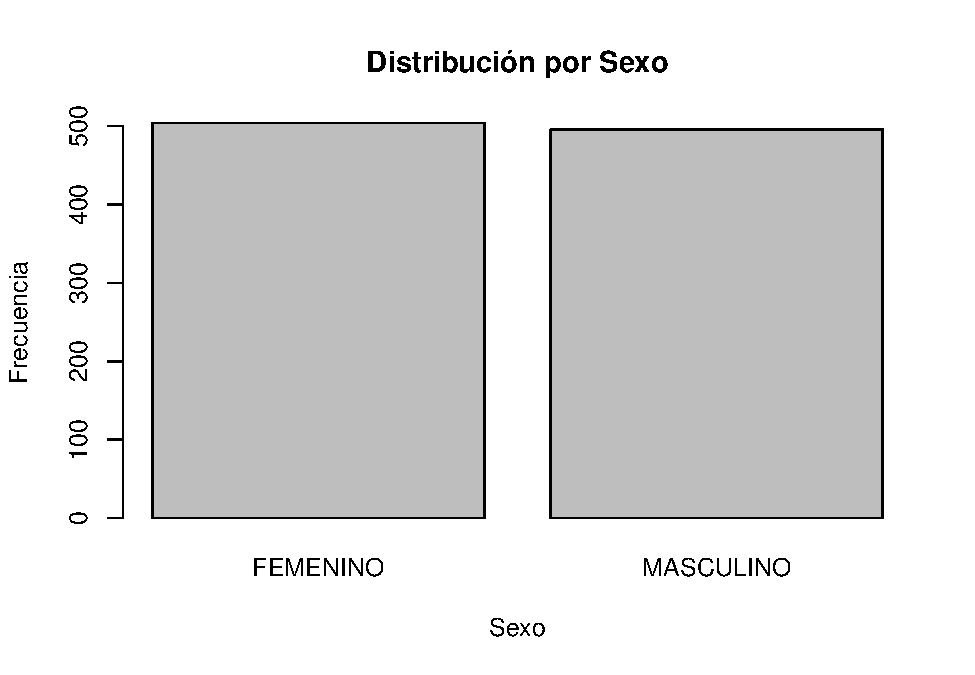
\includegraphics{bookdown-demo_files/figure-latex/analisisdesc-1.pdf} 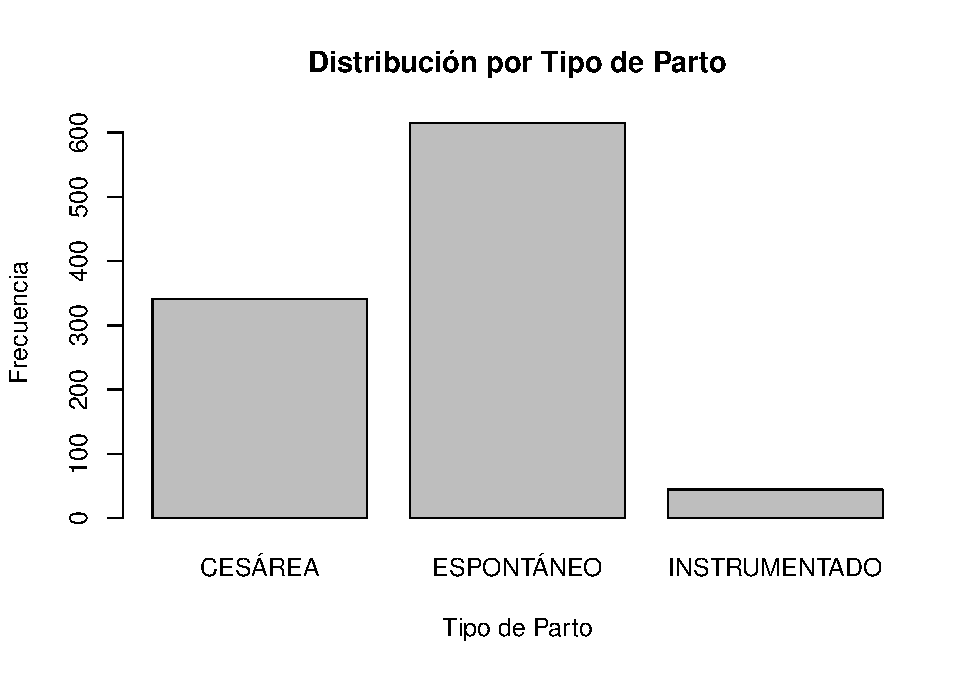
\includegraphics{bookdown-demo_files/figure-latex/analisisdesc-2.pdf} 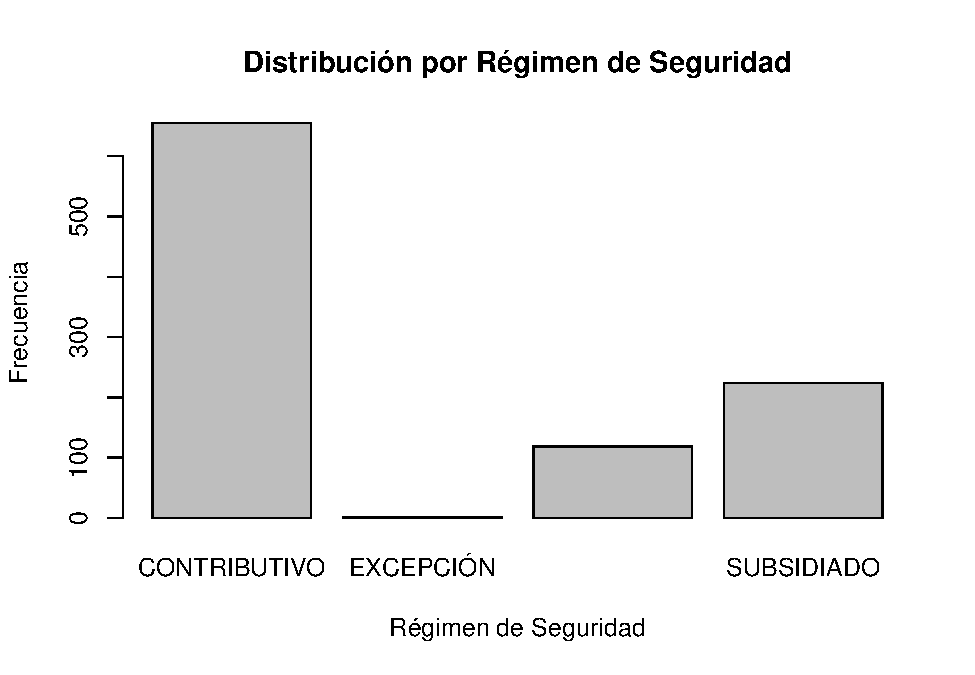
\includegraphics{bookdown-demo_files/figure-latex/analisisdesc-3.pdf} 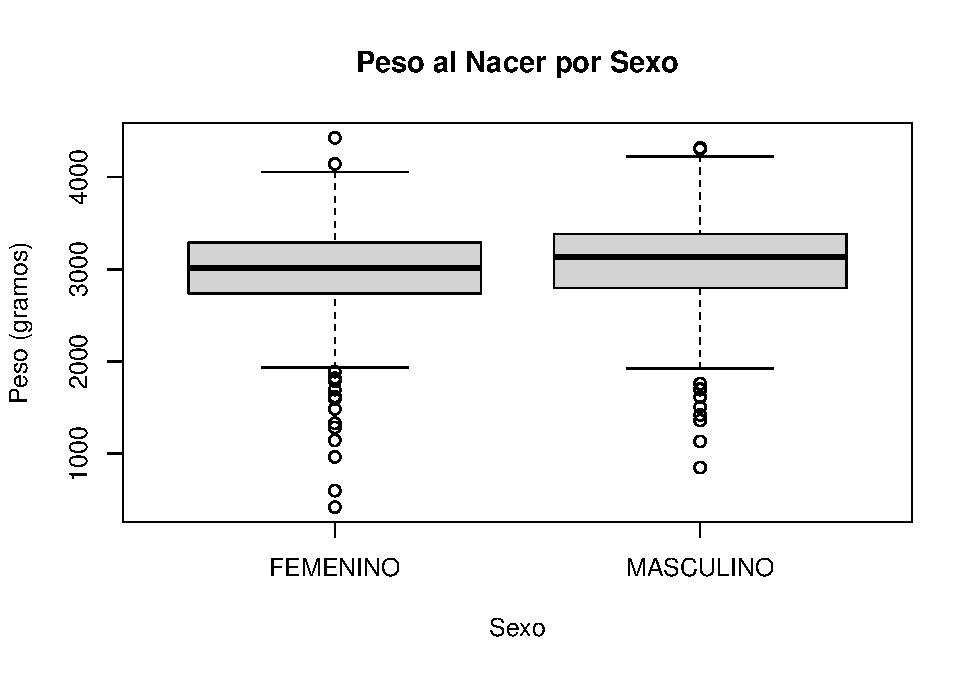
\includegraphics{bookdown-demo_files/figure-latex/analisisdesc-4.pdf} 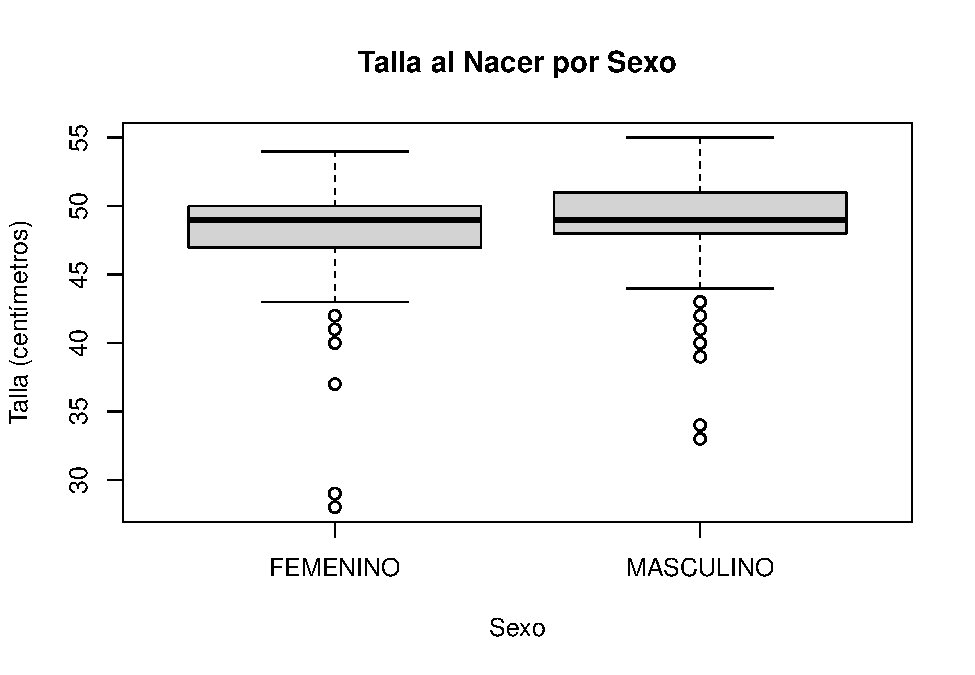
\includegraphics{bookdown-demo_files/figure-latex/analisisdesc-5.pdf}

Después de realizar un análisis descriptivo de algunas variables clave en el conjunto de datos, podemos llegar a varias conclusiones importantes:

\begin{enumerate}
\def\labelenumi{\arabic{enumi}.}
\item
  \textbf{Peso al nacer}: El peso promedio al nacer es de aproximadamente 3023 gramos, con un rango que va desde 420 gramos hasta 4425 gramos. La mayoría de los bebés tienen un peso al nacer que oscila entre 2754 gramos y 3336 gramos, como lo indica el primer y tercer cuartil respectivamente.
\item
  \textbf{Talla al nacer}: La talla promedio al nacer es de alrededor de 48.83 centímetros, con un rango que va desde 28 centímetros hasta 55 centímetros. La mayoría de los bebés tienen una talla al nacer que oscila entre 48 y 50 centímetros, como lo indica el primer y tercer cuartil respectivamente.
\item
  \textbf{Tiempo de gestación}: El tiempo promedio de gestación es de aproximadamente 38.17 semanas, con un rango que va desde 25 semanas hasta 41 semanas. La mayoría de las gestaciones tienen una duración que oscila entre 37 y 39 semanas, como lo indica el primer y tercer cuartil respectivamente.
\item
  \textbf{Edad de la madre}: La edad promedio de la madre es de alrededor de 27.04 años, con un rango que va desde 13 años hasta 46 años. La mayoría de las madres tienen una edad que oscila entre 23 años y 32 años, como lo indica el primer y tercer cuartil respectivamente.
\end{enumerate}

  \bibliography{book.bib,packages.bib}

\end{document}
